\documentclass[12pt]{beamer}
\usetheme{Madrid}
\usepackage[utf8]{inputenc}
\usepackage[spanish]{babel}
\usepackage{amsmath}
\usepackage{amsfonts}
\usepackage{amssymb}
\usepackage{multicol}
\usepackage{graphicx}
\graphicspath{ {./images/} }

\author[Edgar, Shah, Ronald]{Edgar Luque \and Shah Sawar \and Ronald Intriago}
\title{Gymodo}
\subtitle{La mejor app para tu gym} 


\definecolor{gymodo_orange}{rgb}{1, 0.556, 0.235}

\definecolor{UBCblue}{rgb}{0.04706, 0.13725, 0.26667}
\usecolortheme[named=UBCblue]{structure}

%\setbeamercovered{transparent} 
%\setbeamertemplate{navigation symbols}{} 
\logo{
\includegraphics[height=1cm]{gymodo_logo}} 
\institute[2WIAM]{
Proyecto de Desarrollo de Aplicaciones Multiplataforma \\
2WIAM \\
Escola del Treball de Barcelona
} 
\date[17-05-2021]{17 de mayo de 2021} 

\begin{document}

\begin{frame}
\titlepage
\end{frame}

\begin{frame}
\frametitle{Índice}
\tableofcontents
\end{frame}

\section{Abstract}
\begin{frame}{Abstract}

\textbf{\color{gymodo_orange} Gymodo} es una aplicación que tiene como objetivo resolver los problemas que puedan tener los gimnasios en estos tiempos modernos, pero sobre todo, problemas originados a partir de la pandemia del Covid-19.

\begin{itemize}
\item Reservar hora en el gimnasio
\item Crear workouts
\item Crear dietas, escaneando los productos
\item Ver noticias
\item Publicar publicaciones con comentarios, una mini red social
\end{itemize}

\end{frame}

\section{Visualización de la app}
\begin{frame}{Visualización de la app}

\only<1> {

\begin{center}
\includegraphics[width=0.23\textwidth]{gymodo_home}
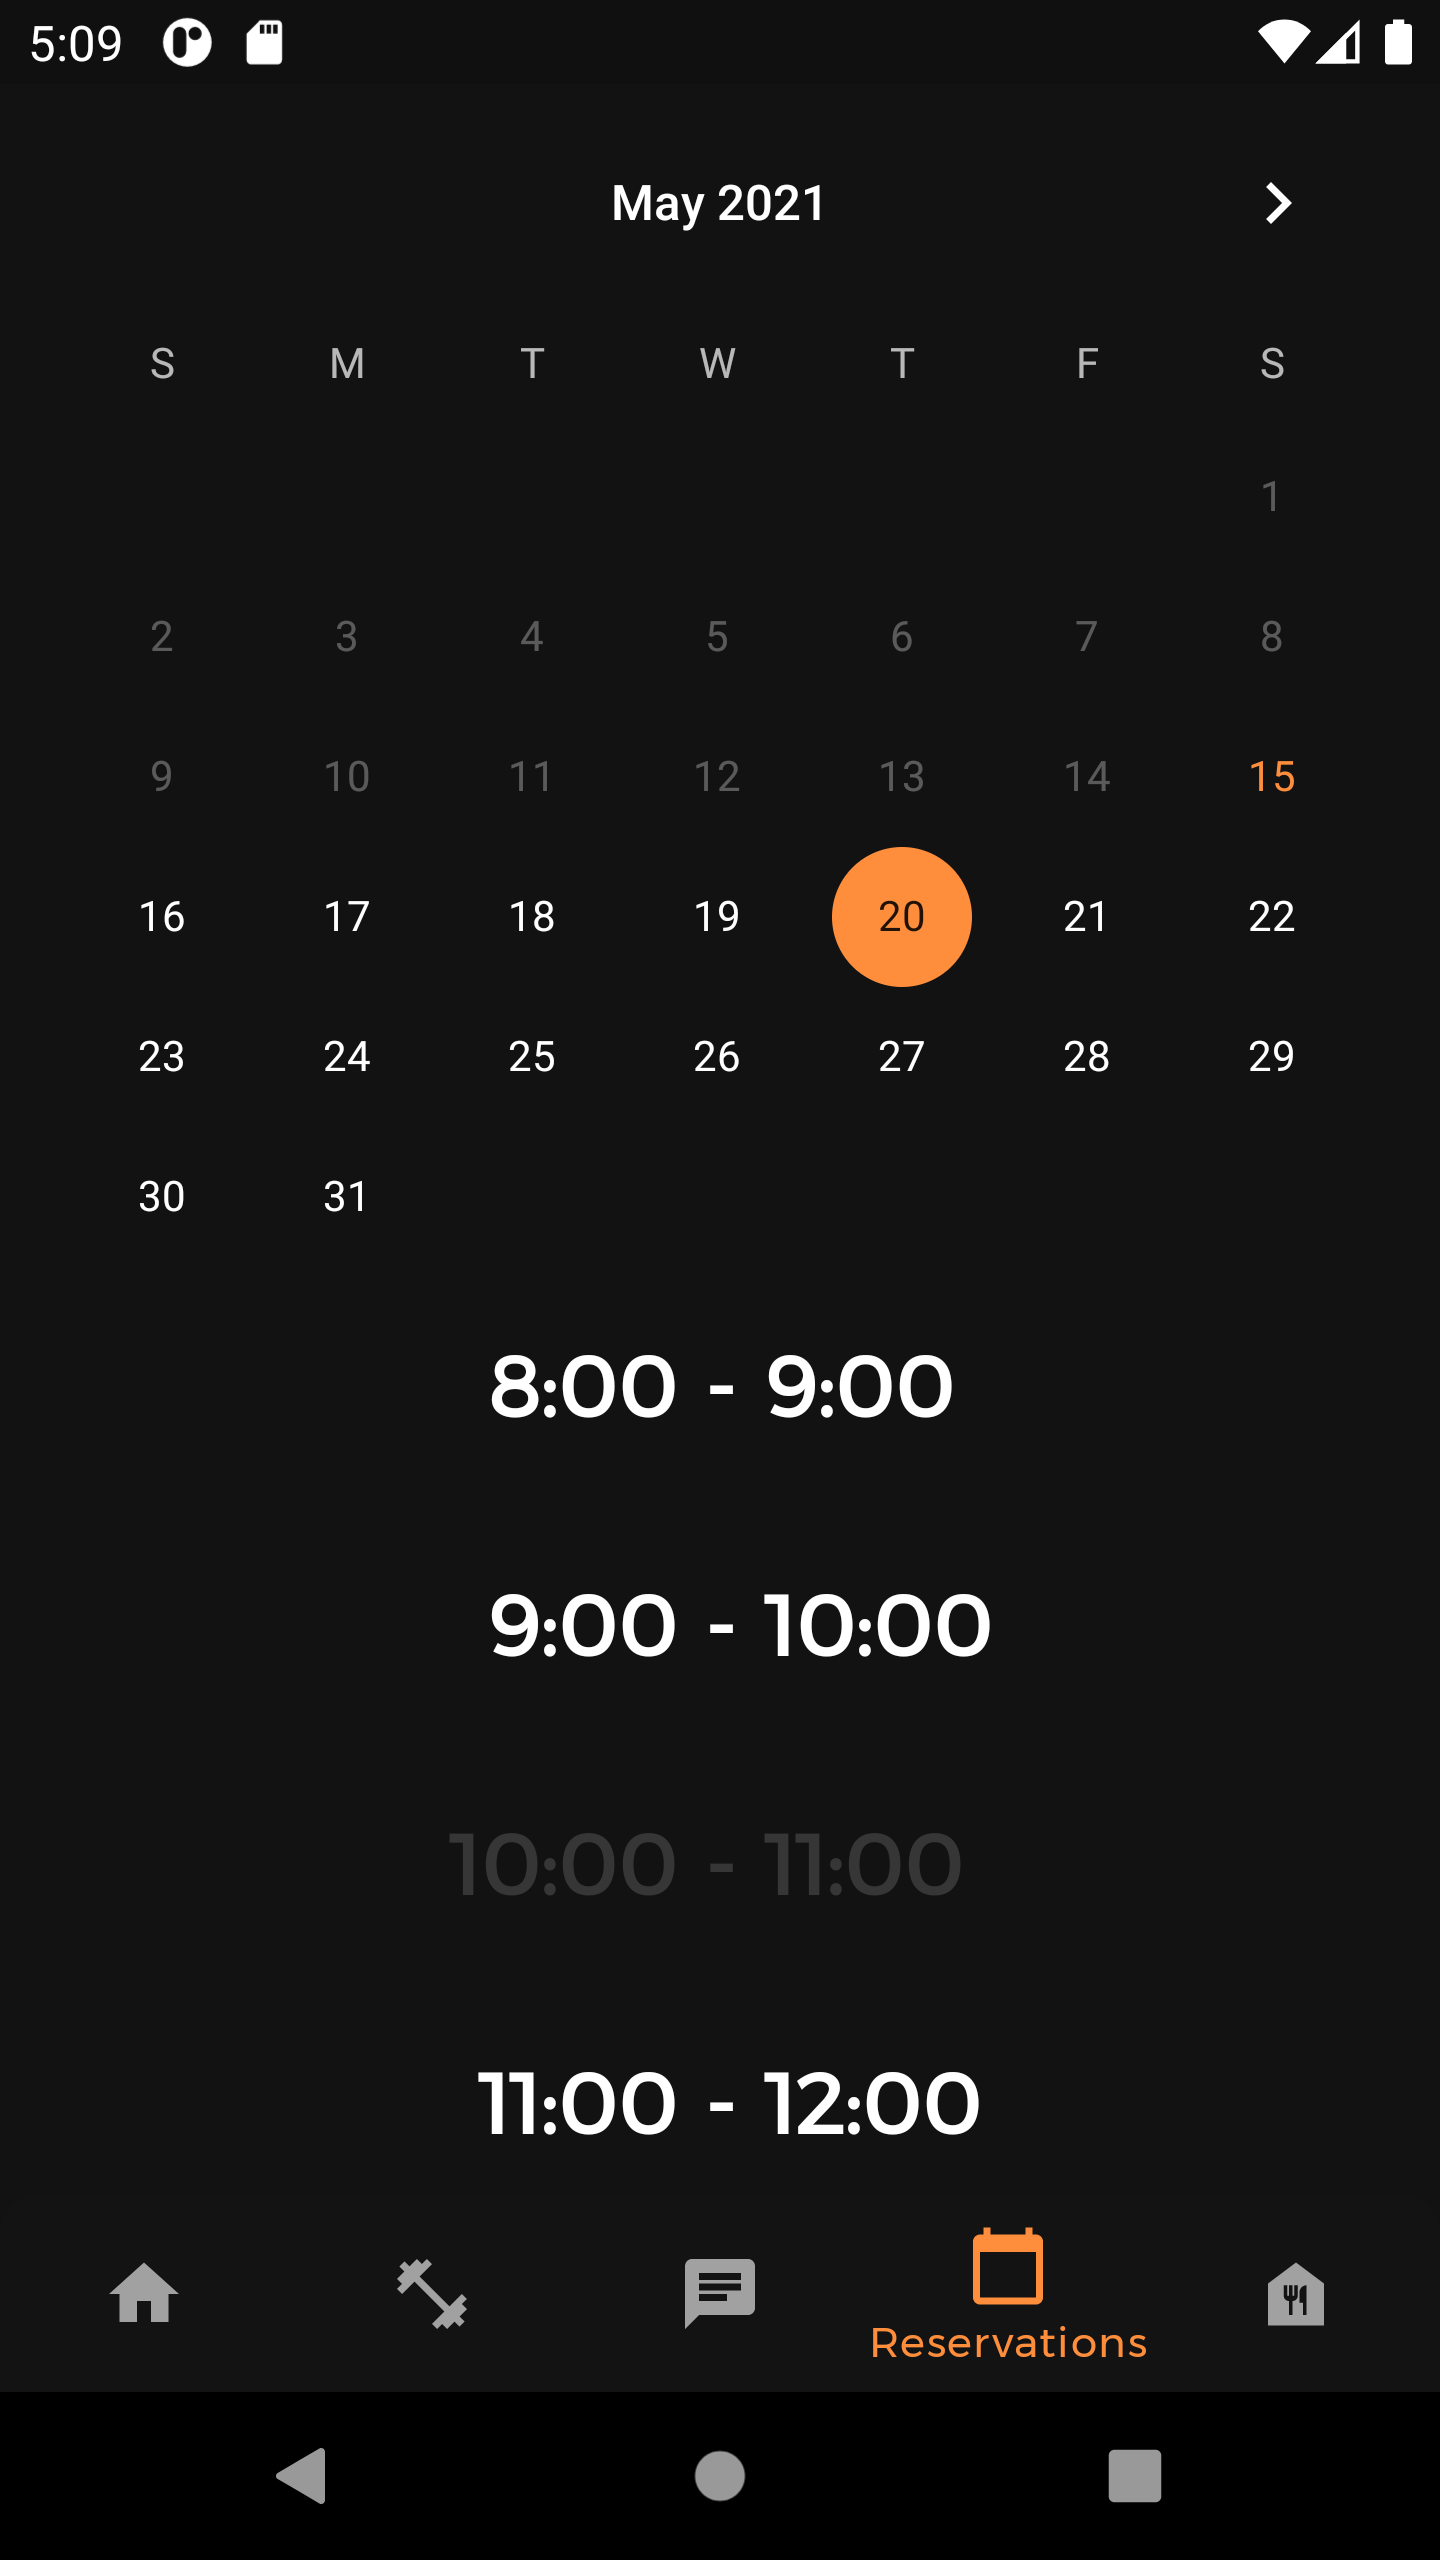
\includegraphics[width=0.23\textwidth]{gymodo_create_reservation}
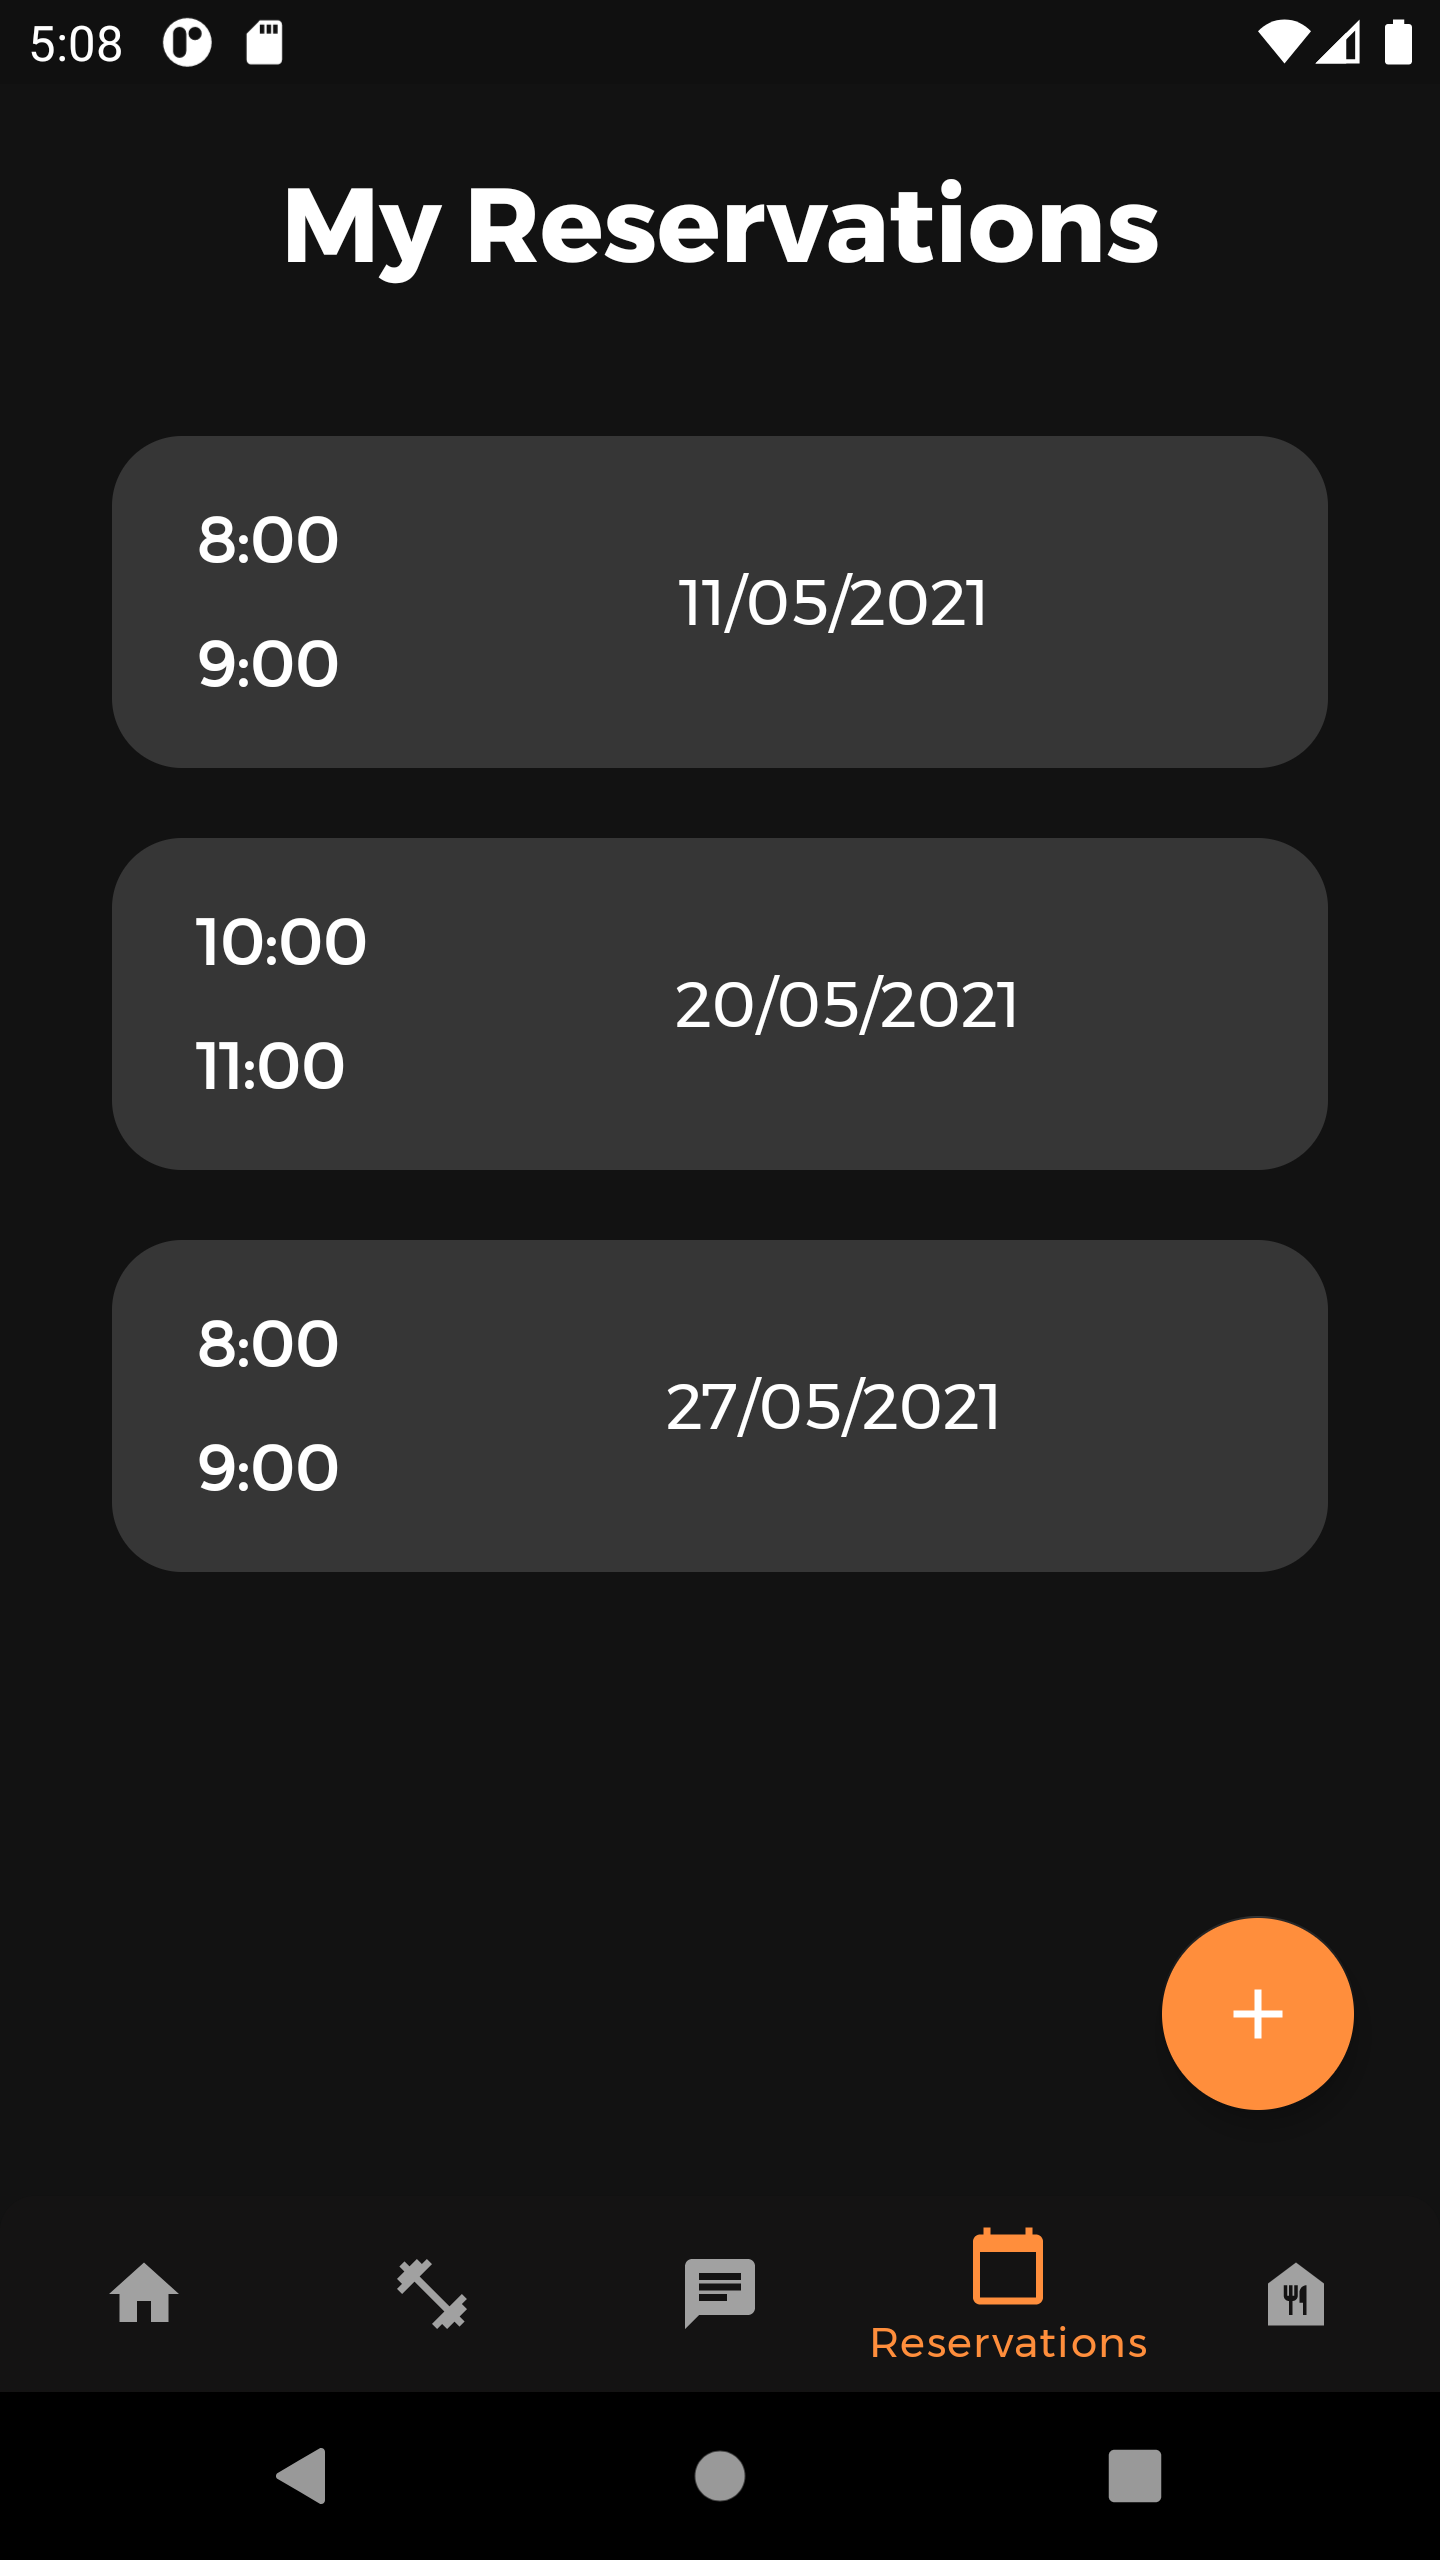
\includegraphics[width=0.23\textwidth]{gymodo_your_reservations}
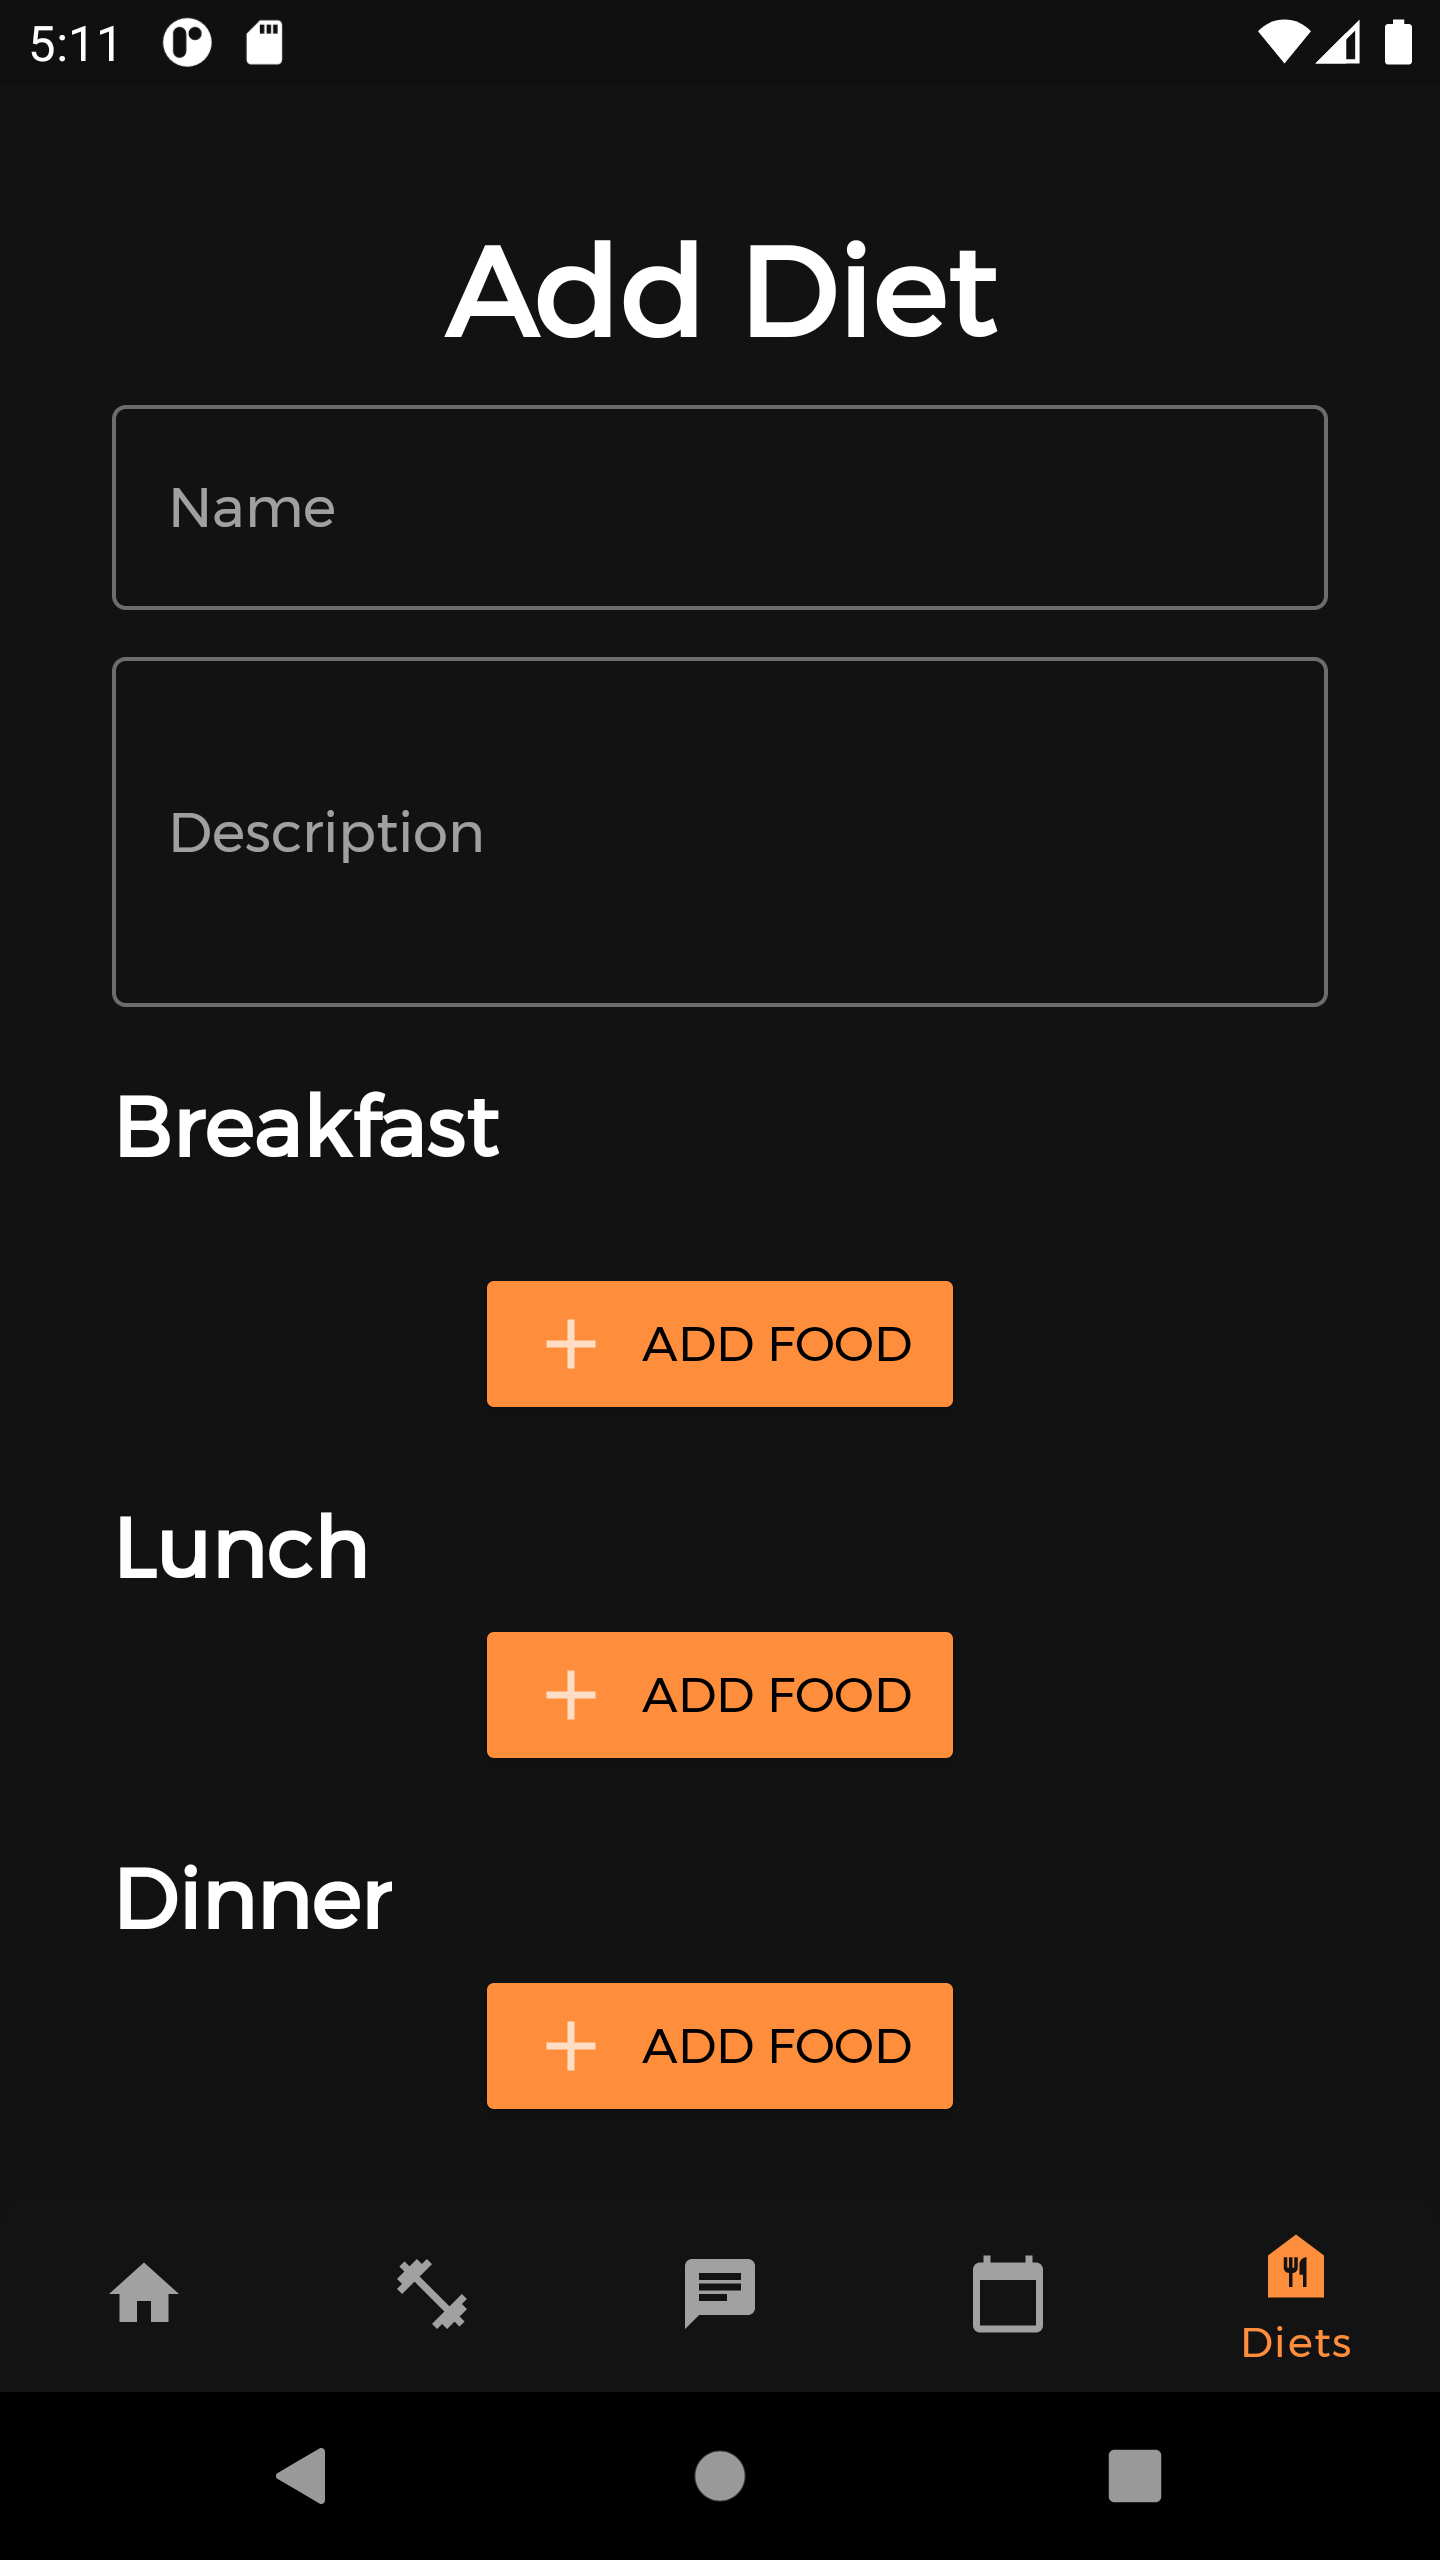
\includegraphics[width=0.23\textwidth]{gymodo_add_diet}
\end{center}

}

\only<2> {

\begin{center}
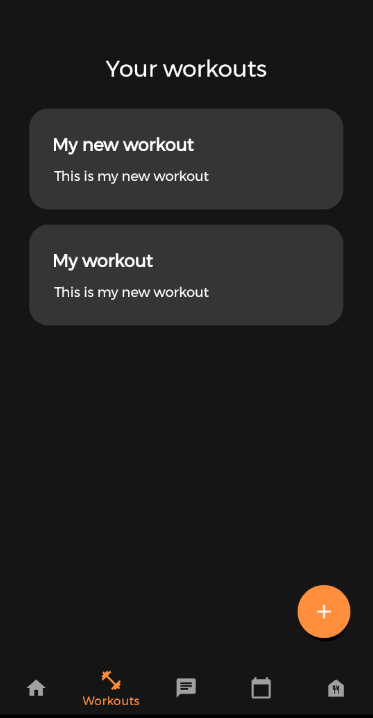
\includegraphics[width=0.23\textwidth]{pres_1}
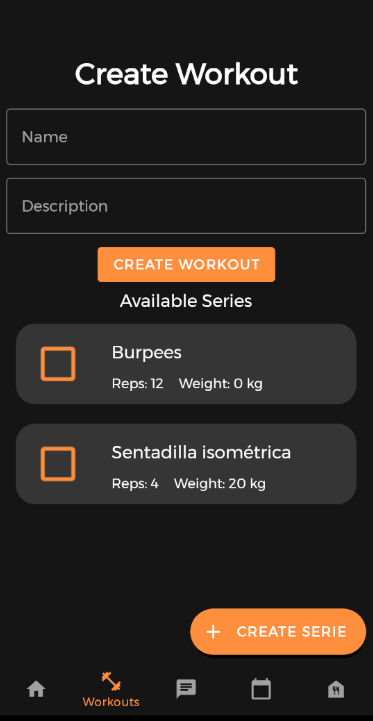
\includegraphics[width=0.23\textwidth]{pres_2}
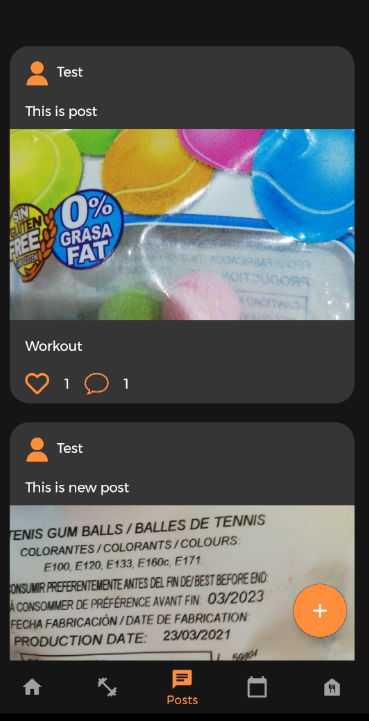
\includegraphics[width=0.23\textwidth]{pres_3}
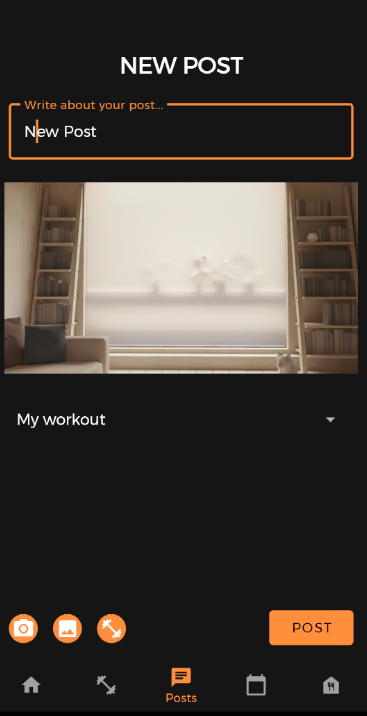
\includegraphics[width=0.23\textwidth]{pres_4}
\end{center}
}


\end{frame}

\section{Tecnología Usada}
\begin{frame}{Tecnología Usada}

\begin{center}


\includegraphics[width=0.2\textwidth]{asana}

\includegraphics[width=0.2\textwidth]{mlkit}

\includegraphics[width=0.2\textwidth]{androidstudio}


\includegraphics[width=0.2\textwidth]{firebase}

\includegraphics[width=0.2\textwidth]{toggl}

\includegraphics[width=0.2\textwidth]{git}
{\LARGE \LaTeX}
\end{center}
\end{frame}

\section{Diseño}
\begin{frame}{Diseño}

\begin{center}
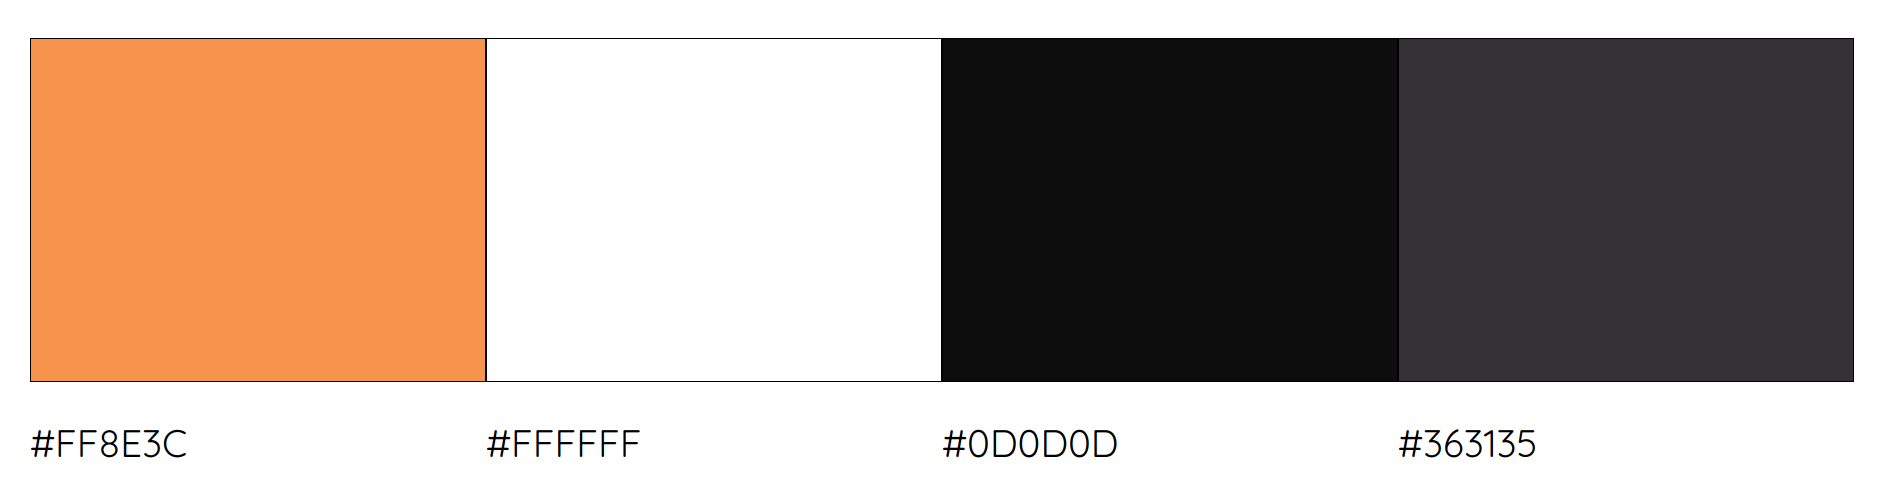
\includegraphics[width=\textwidth]{color_palette}

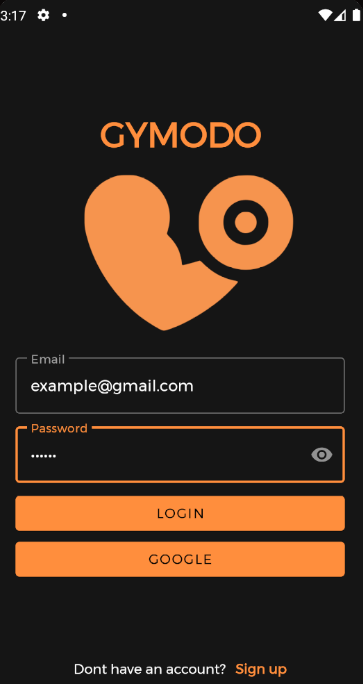
\includegraphics[height=0.45\textheight]{loginconcredenciales}

\includegraphics[width=0.4\textwidth]{gymodo_logo}
\end{center}


\end{frame}

\section{Fases del desarrollo}
\begin{frame}{Fases del desarrollo}

\begin{enumerate}
\item Diagramas:

\begin{itemize}
\item Diagrama de Clases.
\item Diagrama E-R.
\item Casos de uso.
\end{itemize}

\item Mockup del diseño.

\item Configurar el firebase.

\item Crear las clases a partir del diagrama de clases.

\item Crear los layouts (diseño).

\item Implementar la funcionalidad de las views.

\item Crear la documentación.

\end{enumerate}
\end{frame}

\section{Estadísticas}
\begin{frame}{Estadísticas}

\only<1> {
\framesubtitle{Toggl}
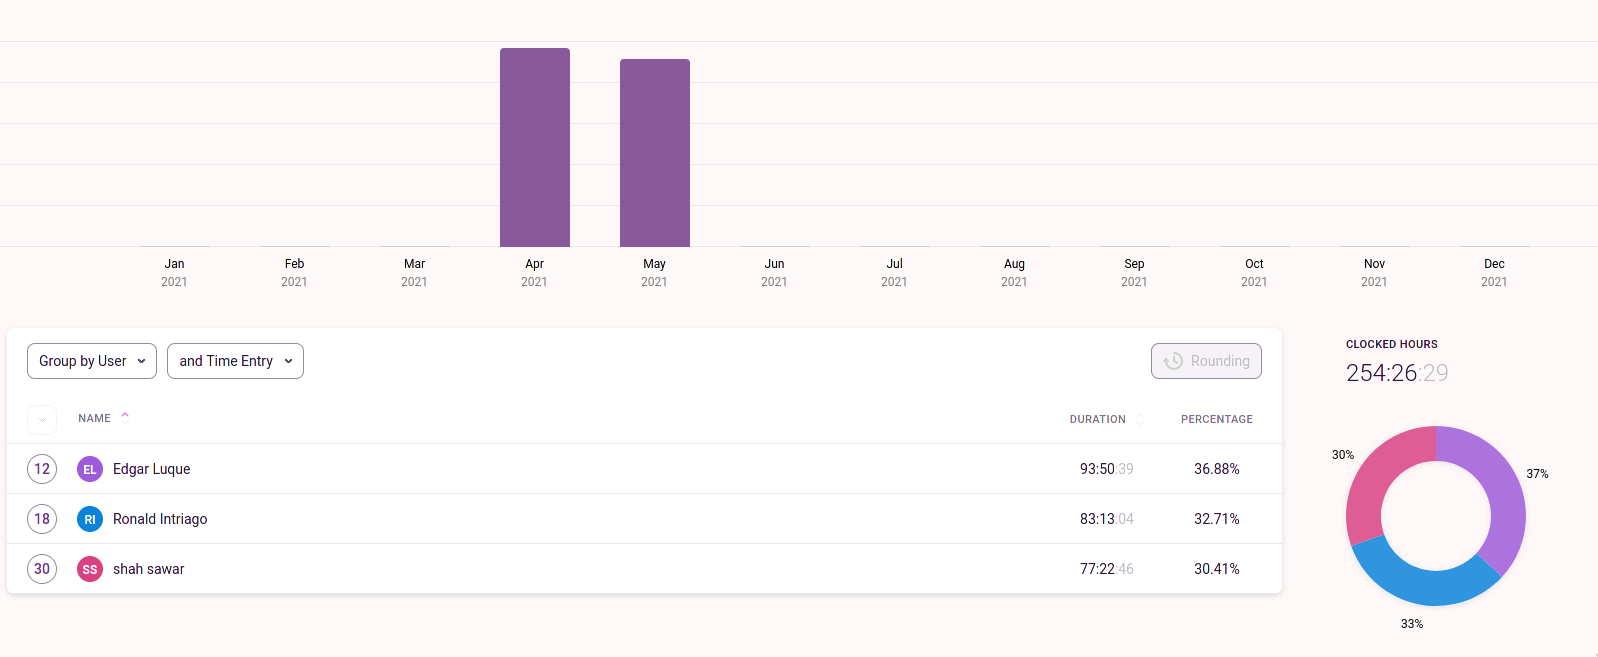
\includegraphics[width=\textwidth]{toggl-stats}
}

\only<2> {
\framesubtitle{Github}

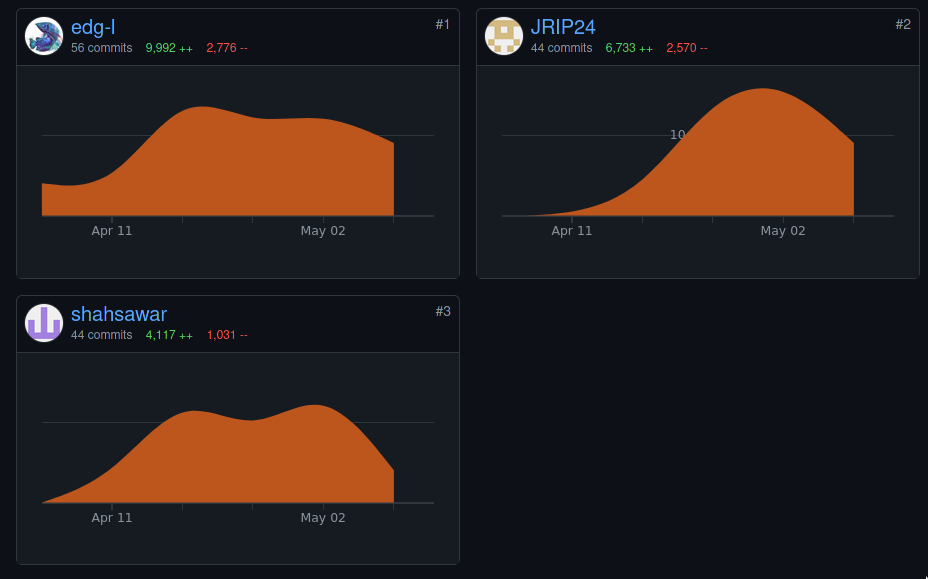
\includegraphics[width=0.92\textwidth]{git-contributors}
}

\end{frame}


\section{Conclusión}
\begin{frame}{Conclusión}

Que hemos aprendido:

\begin{itemize}
\item Git
\item Android
\item Firebase
\item \LaTeX
\item Trabajo en equipo
\end{itemize}


\end{frame}

\section{Preguntas}
\begin{frame}{Preguntas}

\begin{center}

\includegraphics[width=0.8\textwidth]{gymodo_logo}
\end{center}


\end{frame}

\end{document}